\documentclass[t,dvipsnames]{beamer}

\usepackage{c-base-slides}

\usepackage{fancyhdr}
\usepackage{booktabs}
\usepackage{microtype}
\usepackage{amsmath}
\usepackage{amssymb}
\usepackage{mathtools}
\usepackage{nicefrac}
\usepackage{icomma}
\usepackage{tabularx}
\usepackage{svg}
\usepackage{subcaption}
\usepackage{mdframed}


\usepackage{standalone}
\usepackage{tikz}
\usetikzlibrary{decorations, decorations.text,}

\usepackage{pst-solides3d}

% \usepackage[hidelinks]{hyperref}

\usepackage{cleveref}


\usepackage{fontspec}
% % \setmainfont{ceva-c2.ttf}
\setmainfont{Alegreya Sans}

\usepackage{lettrine}
 
\usepackage{biblatex}
\addbibresource{literature.bib}

\definecolor{eins}{HTML}{e7e7e8}   %% Ring 1 "core"     - weiß - Mittelpunkt, Ring um Mittelpunkt
\definecolor{zwei}{HTML}{ed1c24}   %% Ring 2 "com"      - rot -  "Fenster" innen
\definecolor{drei}{HTML}{fbad18}   %% Ring 3  "culture" - orange - fünf Module, quasi invertiert
\definecolor{vier}{HTML}{74c043}   %% Ring 4  "creactive" - grün -  vier Module
\definecolor{fuenf}{HTML}{0089d0}  %% Ring 5 "cience"  - cyan (blau) - drei Module mit "Strich"
\definecolor{sechs}{HTML}{11357e}  %% Ring 6 "carbon" -  indigo - viele "Fenster" außen
\definecolor{sieben}{HTML}{000000} %% Ring 7 "clamp" -  schwarz, c-förmig
\definecolor{cbase}{HTML}{222222}  %% Körper der Raumstation


\newcommand{\Hrule}[1][.]{%
\begingroup\color{#1}%
    \resizebox{\textwidth}{!}{
    
\begin{tikzpicture}
        \filldraw[draw=black]  (0,0) rectangle (10,0.2);
    \end{tikzpicture}
    }%
\endgroup%
}

\newcommand{\Hrulek}[1][.]{%  used in table
\begingroup\color{#1}%
    \resizebox{3ex}{!}{
    
\begin{tikzpicture}
        \filldraw[draw=black]  (0,0) rectangle (2,1);
    \end{tikzpicture}
    }%
\endgroup%
}

\newcommand{\ceva}[1]{ % Leerzeichen notwendig
    {\fontspec{[ceva-c2.ttf]}#1}%
}
\newcommand{\cevain}[1]{ % Leerzeichen notwendig!
    {\fontspec{[ceva-c2.ttf]}#1} $\mid$ \emph{#1}%
    \index{{\fontspec{[ceva-c2.ttf]}#1} $\mid$ #1}%
}
% \newcommand{\cevalong}[1]{ {\fontspec{[ceva-c2.ttf]}#1} | \emph{#1}}

\newcommand{\ring}[1]{ % Leerzeichen notwendig
    {\fontspec{[ceva-c2.ttf]}#1}%
    % \index{{\fontspec{[ceva-c2.ttf]}#1} $\mid$ #1}
}

\newcommand{\twofonts}[2][]{
\begin{quote} 
    {\fontspec{[ceva-c2.ttf]}#2}
    \par
    #2\hfill#1
\end{quote}
}

\newcommand{\linek}[2][]{
\begin{quote} 
    {\fontspec{[linek.ttf]}#2}
    \par
    {\fontspec{[ceva-c2.ttf]}#2}
    \par
    #2\hfill#1
\end{quote}
}
\newcommand{\linekin}[1]{ % Leerzeichen notwendig!
    {\fontspec{[linek.ttf]}#1} $\cdot$ %
    {\fontspec{[ceva-c2.ttf]}#1} $\mid$ \emph{#1}%
    \index{{\fontspec{[linek.ttf]}#1} $\cdot$ {\fontspec{[ceva-c2.ttf]}#1} $\mid$ #1}%
}


\newenvironment{newstuff}
{}
{\hfill{\footnotesize{[penta]}}
\clearpage
}



\title{topologie der c-base}
\author{penta}
% \date{February 2024}

\begin{document}

\frame{\titlepage}


\begin{frame}{Ursprungsmythos}
        \twofonts[\cite{cbasefund}]{
    an einem verregneten nachmittag im august 1995 stolperte Hardy Krause über ein herumliegendes teil in einem bauschacht nördlich des alexanderplatzes in berlin.
    [...]
    % verärgert trat er nach dem außerordentlich harten objekt, welches ihm innnerhalb der nächsten halben stunde wohl eine schöne beule bescheren würde und fluchte.
    % doch 
    % dann betrachtete er das
    [...]
    % die beule verursachende 
    % stück genauer und bemerkte neben einer revolutionären farbgebung (metallisch-violett) erstaunliches: 
    auf diesem irgendwie nicht in diese umwelt passenden stück schrott waren schriftzeichen eingraviert
    [...]:
    % , die unbedingt einer genaueren untersuchung unterzogen werden mußten.
    % 
    % also grub ein team das fundstück aus und brachten es zu einem befreundeten radiochemiker. mit hilfe des kohlenstoff-14-tests (auch radiocarbon-methode genannt) fand er heraus, daß es, nach irdischem ermessen, mindestens 100.000 (!) jahre alt sein müßte.
    % 
    % außerdem enthielte es ein element mit einer ordnungszahl von über 200, das bisher, selbst mit den besten technischen möglichkeiten nicht herstellbar ist. es ist also älter als jedes bisher gefundene von menschen so kunstvoll bearbeitete metallstück und kann wahrscheinlich erst irgendwann in der fernen zukunft enstanden sein!?!

    % auf seiner oberfläche sind zudem irdische schriftzeichen eingraviert
    
    c-base project - be future compatible.
    }
\end{frame}

\begin{frame}{The Motto}
        Eingraviert in die Oberfläche des \ceva{urartefact} ist nach dieser Quelle die Inschrift 
        
    \linek[\cite{cbasefund}]{c-base project - be future compatible}  
    
    Hier wird der Gedanke einer Vorwärtskompatiblität (\linekin{future compatible}) statt Rückwärtskompatiblität ausgedrückt. Wer diesem Ruf folgt, der richtet sein Handeln so ein, dass alles aus ihm hervorgehende Sein \linekin{be} soweit irgend möglich kompatibel zur Zukunft ist, also mit ihr und in ihr funktioniert.
\end{frame}

\begin{frame}{Periodisierung}
    \resizebox{!}{0.8\textheight}{
    \documentclass{standalone}
\usepackage{tikz}
\usepackage{fontspec}

\newcommand{\ceva}[1]{ {\fontspec{[ceva-c2.ttf]}#1}}
\newcommand{\cevain}[1]{ {\fontspec{[ceva-c2.ttf]}#1} | \emph{#1}}

\begin{document}
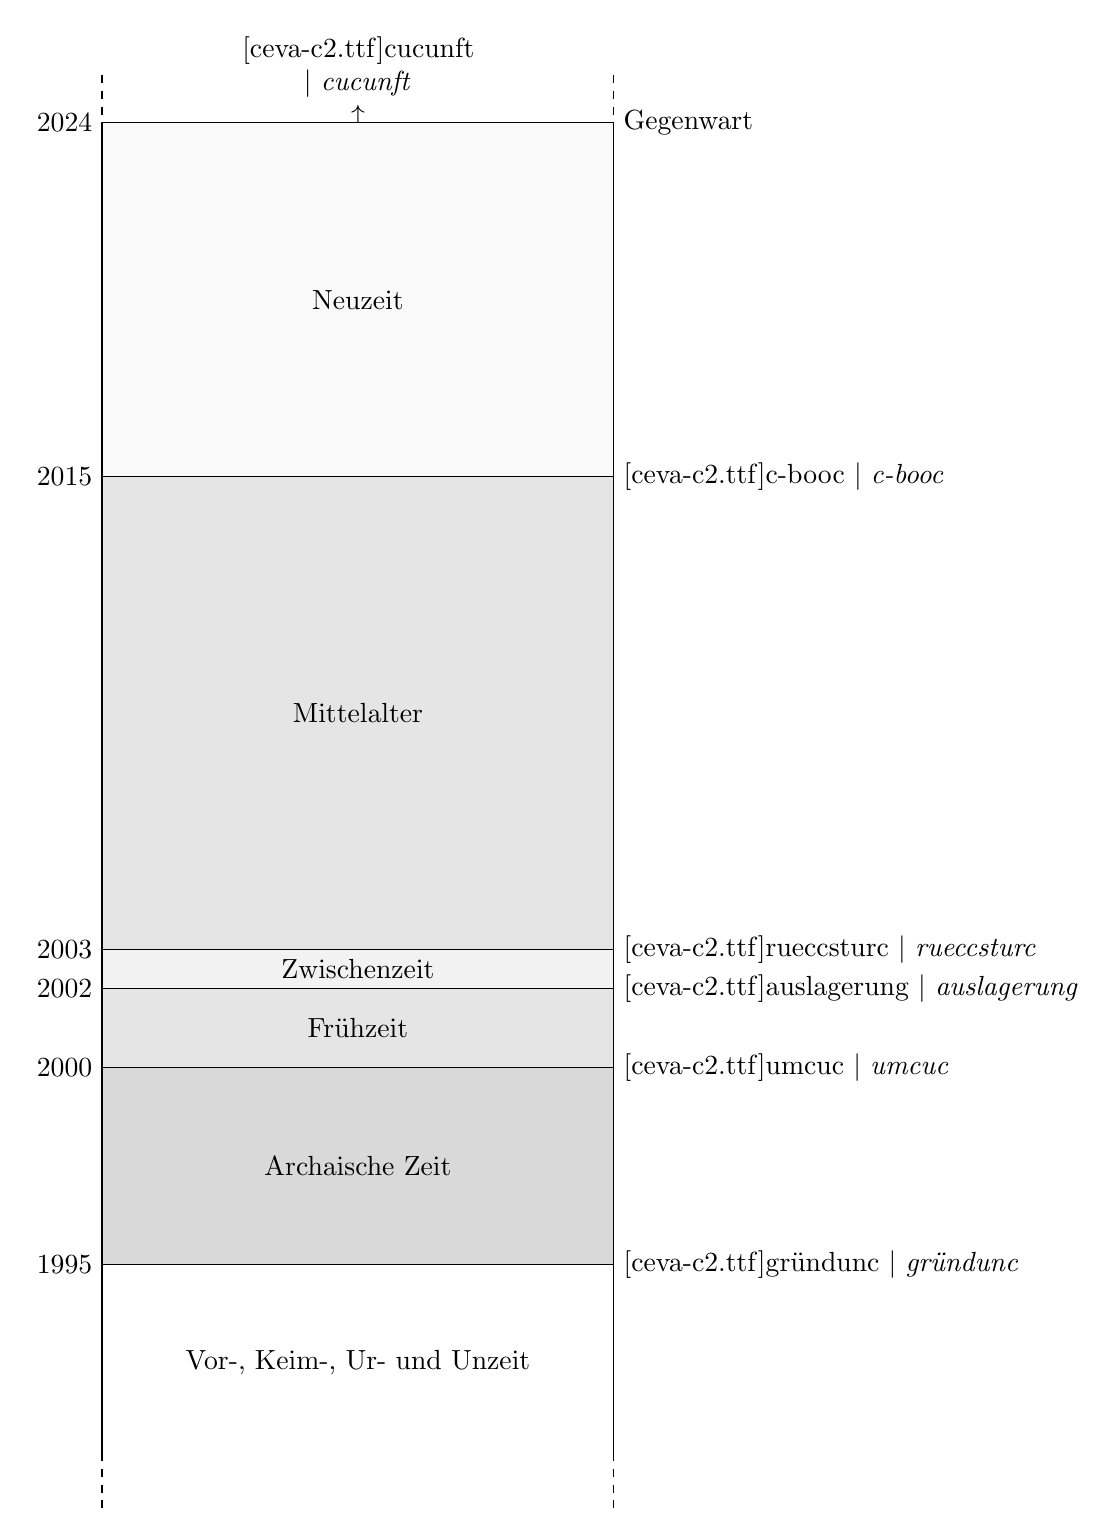
\begin{tikzpicture}[yscale=0.5,xscale=1.3]
    % \draw (0) rectangle (0,,1);
    \foreach \i in {124.4,124.8,125.2} 
        {
        \draw (0,\i) -- (0,\i-0.2);
        \draw (5,\i) -- (5,\i-0.2);
        }

    \node at (2.5,125) {\parbox{20ex}{\centering\cevain{cucunft}\\ $\uparrow$ }};
    
    \node [right] at (5,124) {Gegenwart};
    
    \draw[fill=gray!5] (0,124) node [left] {2024} rectangle node {Neuzeit} (5,115) node [right] {\cevain{c-booc}};
    % \draw (0,115) -- (0,124); draw (5,114) -- (5,124); \draw (0,115
    
    \draw[fill=gray!20] (0,115) node [left] {2015} rectangle node {Mittelalter} (5,103) node [right] {\cevain{rueccsturc}};
    
    \draw[fill=gray!10] (0,103)  node [left] {2003} rectangle node {Zwischenzeit} (5,102) node [right] {\cevain{auslagerung}};
    
    \draw[fill=gray!20] (0,102)  node [left] {2002} rectangle node {Frühzeit} (5,100) node [right] {\cevain{umcuc}};
    
    \draw[fill=gray!30] (0,100)  node [left] {2000} rectangle node {Archaische Zeit} (5,95) node [right] {\cevain{gründunc}};
    % \node at (0,95) [left] {1995};
    
    \draw[draw=none] (0,95)  node [left] {1995} rectangle node {Vor-, Keim-, Ur- und Unzeit} (5,90) ;
    \draw (0,95) -- (0,90); \draw (5,95) -- (5,90);
    
    \foreach \i in {89.8,89.4,89} 
        {
        \draw (0,\i) -- (0,\i-0.2);
        \draw (5,\i) -- (5,\i-0.2);
        }
    
    
    % \draw[<->] (0,95) rectangle (0,65);
\end{tikzpicture}

\end{document}

    }
\end{frame}

\begin{frame}{Die kanonischen Schriften}
    \resizebox{\textwidth}{!}{
        \begin{tabular}{r|lrl}
        \toprule
        \multicolumn{2}{c}{Quelle} & Jahr & Epoche \\
        \midrule
         \ceva{c-booc} & c-booc & 2015 & Übergang Mittelalter$\rightarrow$Neuzeit\\
         \ceva{c-tour} & c-tour & 2006 & frühes Mittelalter \\
         \ceva{starbase-manual7} & starbase-manual7 & 2003 & Frühzeit (?) \\
         \ceva{logbuch now} & logbuch now & 2000 & Archaik\\
         \ceva{logbuch pre} & logbuch pre & 1995 & Archaik, Vorzeit \\
         \bottomrule
    \end{tabular}
    }
\end{frame}

\begin{frame}[allowframebreaks]{Textgrundlage}
    \twofonts[\cite{cbasestarbasemanual}]{
    % 1995 wurden unter Berlin-Mitte die Überreste einer 4,5 Milliarden Jahre alten Raumstation entdeckt. 
    Erste Forschungen ergaben, daß sich die c-för\-mi\-ge Raumstation mit ihrem Mittelpunkt unter dem heutigen Alexanderplatz \emph{befinden muß} und aus 7 Ringen besteht.
    % Aufgrund eines Fundstückes mit der Aufschrift "`\emph{c-base - be future compatible}"' und in Anlehnung an die Anzahl der Ringe, legte das anfänglich nur aus wenigen Mitgliedern bestehene Rekonstructionsteam den Projektnamen und die Aufteilung in sieben Arbeitsbereiche fest.
    % 
    % construct: die raumstation besteht aus sieben ringen, zum teil drehbar. insgesamt hat sie einen durchmesser von 1650 metern
        }

    \framebreak

    \twofonts[\cite{cbasestarbasemanual}]{
    % 1995 wurden unter Berlin-Mitte die Überreste einer 4,5 Milliarden Jahre alten Raumstation entdeckt. 
    % Erste Forschungen ergaben, daß sich die c-för\-mi\-ge Raumstation mit ihrem Mittelpunkt unter dem heutigen Alexanderplatz \emph{befinden muß} und aus 7 Ringen besteht.
    Aufgrund eines Fundstückes mit der Aufschrift "`\emph{c-base - be future compatible}"' und in Anlehnung an die Anzahl der Ringe, legte das anfänglich nur aus wenigen Mitgliedern bestehene Rekonstructionsteam den Projektnamen und die Aufteilung in sieben Arbeitsbereiche fest.
    % 
    % construct: die raumstation besteht aus sieben ringen, zum teil drehbar. insgesamt hat sie einen durchmesser von 1650 metern
        }
    
\end{frame}

\begin{frame}{Zwischenergebnis}


\begin{itemize}
    \item Unter Berlin liegen die Überreste einer c-förmig aufgebauten Raumstation, die sich in sieben \ring{ringe} gliedert.
    \item \ring{ringe} sind Aspekte oder Funktionen, die ineinander verschachtelt sind, miteinander kommunizieren, einander brauchen und sich gegenseitig stärken, und erst in zweiter Linie  Orte im Raum.
    \item Sie sind \textbf{nicht} einander ausschließende Kategorien.
    % \item Die kanonische Literatur über diese \ring{ringe} wird im Folgenden wiedergegeben und die Funktion der \ring{ringe} anschließend beschrieben.
    % \item Da unser Fokus auf der Funktion innerhalb des autopoietischen Systems \ceva{c-base} liegt, wird auf eine detaillierte Beschreibung einzelner Projekte, Module, Artefakte, Module und Bewohner wird verzichtet.
    % \item Eine sehr gute Übersicht über ausgewählte einzelne Projekte, Aggregate, Artefakte und Module bietet das kanonische \ceva{c-booc}~\cite{cbasebook}. Zur Funktion, Geschichte und Ausgrabungsgeschichte der Station und des Rolle des Vereins c-base e.V. sei auf die \ceva{Pressemappe}~\cite{cbasepressemap} verwiesen.
\end{itemize}
\end{frame}

\begin{frame}[allowframebreaks]{Die 7 \cevain{Ringe}}

    \begin{tabular}{rlllr}
    \toprule
        1 & \ceva{core} & core & grau / weiß   & \Hrulek[eins]  \\
        2 & \ceva{com} & com & rot   & \Hrulek[zwei] \\
        3 & \ceva{culture} & culture & orange   & \Hrulek[drei] \\
        4 & \ceva{creactive} & creactive & grün  & \Hrulek[vier]  \\
        5 & \ceva{cience} & cience & cyan  & \Hrulek[fuenf]  \\
        6 & \ceva{carbon} & carbon & indigo  & \Hrulek[sechs]  \\
        7 & \ceva{clamp} & clamp  & ultraviolett / schwarz  & \Hrulek[sieben] \\
    \bottomrule
\end{tabular}
    
    \framebreak
    
    \resizebox{!}{0.8\textheight}{
    \input{tikz-ringconvention}
    }

    \framebreak

    \resizebox{!}{0.8\textheight}{
    \input{tikz-c-base}
    }
\end{frame}


\begin{frame}{Verflachung}

    Die aktuelle Form ist Folge des den Absturzes der Raumstation, und vermutlich ist die gewissermaßen "`flache"' Struktur, die wir bei den bisherigen Rekonstruktionsphasen ausgemacht haben, eine zweidimensionale Projektion der eigentlich mehrdimensionalen Raumstation. 
    
    Diese Frage stellt sich: welche Topologie hatten die \ring{ringe}, welche Topologie hatte die Station vor dem Absturz, und welche strebt sie damit an??
    
    % \paragraph{Ringförmige Anordnung der Ringe}
    Wir haben gesehen, dass sich \ceva{clamp} und \ceva{core} berühren bzw. über eine Einstein-Rosen-Brücke verbunden sind. Daraus folgern wir eine (ursprünglich, zukünftig) \emph{ringförmige Anordnung der Ringe.}  

\end{frame}

\begin{frame}{Ringförmige Anordnung der \ring{ringe}}
    \resizebox{!}{0.8\textheight}{
     \documentclass{standalone}
\usepackage{tikz}
\usetikzlibrary{decorations, decorations.text}
\usepackage{calc}
\usepackage{xcolor}
\usepackage{fontspec}
\newcommand{\ceva}[1]{~{\fontspec{[ceva-c2.ttf]}#1}}
\definecolor{eins}{HTML}{e7e7e8}   %% Ring 1 "core"     - weiß - Mittelpunkt, Ring um Mittelpunkt
\definecolor{zwei}{HTML}{ed1c24}   %% Ring 2 "com"      - rot -  "Fenster" innen
\definecolor{drei}{HTML}{fbad18}   %% Ring 3  "culture" - orange - fünf Module, quasi invertiert
\definecolor{vier}{HTML}{74c043}   %% Ring 4  "creactiv" - grün -  vier Module
\definecolor{fuenf}{HTML}{0089d0}  %% Ring 5 "cience"  - cyan (blau) - drei Module mit "Strich"
\definecolor{sechs}{HTML}{11357e}  %% Ring 6 "carbon" -  indigo - viele "Fenster" außen
\definecolor{sieben}{HTML}{000000} %% Ring 7 "clamp" -  schwarz, c-förmig
\definecolor{cbase}{HTML}{222222}  %% Körper der Raumstation    
\begin{document}
%% c-base logo nachgebaut von penta.
%% alles nur geschätze Winkel und Abstände :/
%% um den code zu verstehen, einfach mal einzelne Teile auskommentieren und wieder einkommentieren (ctrl-#) und dann mal \draw[white] durch \draw[red] ersetzen, dann sieht man, was was ist.
%% viel Spaß damit.
\tikzset{
  pics/carc/.style args={#1:#2:#3:#4}{
    code={
      \draw[postaction={decorate, decoration={text along path, raise=-2pt, text align={align=center}, text={\ceva{#4}}, reverse path}}] (#1:#3) arc(#1:#2:#3);
    }
  }
}%
    \begin{tikzpicture}
        \draw[gray, line width=50pt] (0:0) circle (3);
        \foreach [count=\i] \ring/\color in
            {core/eins,com/zwei,culture/drei,creactiv/vier,cience/fuenf,carbon/sechs,clamp/sieben}
            {%
                \draw[color=\color!50,line width=45pt] (0:0) pic{carc=\i*51.418-25:\i*51.418+25:3:\ring};
            }%
    \end{tikzpicture}
\end{document}

    }
\end{frame}

\begin{frame}[allowframebreaks]{Rotationtorus}
    
    Eine \emph{ringförmige Anordnung von Ringen }ist topologisch darstellbar als Fläche, die entsteht, wenn ein Kreis um einen Kreis (also quasi ein \ring{ring} um einen \ring{ring}) rotiert. Diese Figur ist der \emph{Rotationstorus}.

    \framebreak
    \resizebox{!}{0.8\textheight}{
    \input{tikz-torus-white}
    }
     % {Toroidales Polyeder imt $14\times 14$T Flächen} Es hat 14  Meridiane und 14 Parallelkreise (angenähert)

\end{frame}

\begin{frame}{Toroidalinterpretation}
    Grundsätzlich sind die \ring{ringe} Kreisscharen. Es gibt drei unterscheidbare Gruppen von Kreisscharen auf einem Torus: 
    \begin{enumerate}
        \item Parallelkreise (poloidal)
        \item Merididiane (toroidal) und 
        \item Villarceau-Kreise.
    \end{enumerate}
\end{frame}

\begin{frame}[allowframebreaks]{Parallelkreise}
    

   {Parallelkreise} entstehen durch poloidale Schnitte eines   Torus. 
    Eine solche Anordnung ist denkbar, aber wenig plausibel, da die einzelnen Ringe dann eher Schreiben wären. Auch ist nicht zu erkennen, wie es beim Absturz der Station dann zu einer konzentrischen Anordnung gekommen sein sollte. 

    \framebreak
    
    \resizebox{!}{0.8\textheight}{
        \input{tikz-torus-parallele}
        }
\end{frame}

\begin{frame}[allowframebreaks]{Meridiankreise}

        
  {Meridiankreise} entstehen als toridale Schnitte des Rotationstorus. 
    Eine Anodrnung der \ring{ringe} als Meridiankreise ist möglich.  
    Dabei berühren sich hier im Inneren eben \ceva{core} und \ceva{clamp}; das passt zu unserer Interpretation des Kanons von der Topologie der Station als Torus mit einem innenliegenden Wurmloch. In diesem berühren sich innen \ceva{core} und \ceva{clamp}; außen liegt \ceva{creactiv}.

    \framebreak
    \resizebox{!}{0.8\textheight}{
            \input{tikz-torus-meridiane}
            }
    
\end{frame}



% Da der äußerere Äquator (Meridian) \ceva{creactive} enspricht, bedeutet eine Ausweitung der \ceva{creactivität} ein Anschwellen dieses Torus und somit Wachstum der Station; bildlich entspräche das in etwa der Inflation eines Rettungsrings. Dabei ist zu beachten, dass eine Vergrößerung des rotierenden Kreises ohne gleichzeitige Ausweitung des Rototaionsradius im Torus zu einem Verschwinden des innenliegenden Loches führen könnte. Dann wäre die Station gewissermaßen an ihrer eigenen \ceva{creactivität} erstickt.

% Unsere Darstellung in \cref{fig:torus-meridiane} zeigt die \ring{ringe} als Flächen. Tatsächlich sind sie natürlich selbst von höherer Dimension, also ihrerseits Tori. Es sollte sich wirklich um eine Schar von Tori, gewissermaßen um ein Bündel von Ringen, handeln.

\begin{frame}[allowframebreaks]{Villarcreau-Kreise}
    

    Villarceau-Kreise  entstehen topologisch (paarweise) durch den Schnitt einer doppelberührenden Ebene mit dem Torso.

    \framebreak

    \resizebox{!}{0.8\textheight}{
        \includesvg{Torus-vill-point.svg}
        }
    
\end{frame}

\begin{frame}[allowframebreaks]{Villarcreau-Ringe}
    
    Es lässt sich also eine Schar von Kreisen auf einem Torus finden, die sich nicht schneiden, die perfekt kreisförmig und die untereinander kongruent sind. 
    % \cref{fig:villarceautorous} zeigt eine Annäherung, indem hier ein Torus mit $21\times 21$ Flächen belegt wurde.

    \framebreak
    \resizebox{0.8\textheight}{!}{
                \input{tikz-torus-villarceau-ringe1}            
                }

\end{frame}

\begin{frame}[allowframebreaks]{Verknoteter Torus}
    

    Die Ringe sind auf einem Torus in Form verschlungener Bänder angeordnet. Sie winden sich um das Zentrum des Torus und zugleich um den Körper des Torus selbst. 
    Es gibt keinen \ring{ring}, der einen bevorzugten Ort einnimmt. Da sie kongruent sind, sind sie flächen- und längengleich.

    \framebreak
    
    Wie bereits oben müssen wir uns die Ringe nicht wie abgebildet vorstellen, sondern ihrerseits eher als eigenständige Tori oder Toroide. Ähnlich wie ein Torus (2D, eine Fläche) aus Villacreau-Kreisen "`zusammengesetzt"' vorgestellt werden kann, kann ein Toroid (3D, ein Körper, gewissermaßen ein "`ausgefüllter"' Torus) aus Scharen von Tori "`zusammengesetzt"' bzw. approximiert werden. 

    \framebreak
    
    Wir können uns also die \ring{ringe}  als eigene Tori vorstellen.
    Das setzt allerdings voraus, dass die \ring{ringe} eindeutig abgegrenzt sind gegeneinander: jeder \ring{ring} schließt sich nach einer vollen Umdrehung um die Mittelachse des Torus. 

    \framebreak
    
    % \paragraph{Verknoteter Torus}
    Lässt man diese Bedingung fallen, so kann man sich auch einen Torus vorstellen, bei dem jeder Kreis nach $306^o$ an den jeweils nächsten "`anschließt"', also einen "`verknoteten Torus"' bzw. \cevain{cnoten}.

    \framebreak

    \resizebox{0.8\textwidth}{!}{
            \includegraphics{KnottedTorus.png}
        }

    \framebreak    
    Dann gäbe es genau einen parallelen Schnitt durch den \cevain{cnoten}, der  ein Bild wie oben  abgibt, obwohl alle \ring{ringe} und damit die Station als Ganzes ein einzelner, gewissermaßen siebenfach "`gewickelter"' Torus wäre, nämlich ein Torusknoten.

    \framebreak

    Das erklärt auch die Doppelung der Zahl $7$. Es gibt $7$ \ring{ringe} und (jeweils) $7$ \ceva{deccs}. Eine solche toroidale \ceva{cnoten}-Architektur bietet eine Erklärung für die Quasi-Identität von \ring{ringen} und \ceva{deccs}.

\end{frame}

\begin{frame}{\ceva{core} als Torusknoten}
    

    Angesichts der Bedeutung toroidaler Topologie für Fusionsreaktoren vermuten wir, dass wir hier der Topologie des \ceva{Möbius-band-accelerators} bzw. \ceva{Mino-reactors} bzw. \ceva{Cybernetischen Quecksilber-Reaktors}  auf der Spur sind (vgl.~\cref{sec:core}). \ceva{core} selber ist eine komprimierte Spiegelung der Stationsarchitektur als Ganzes. Hier entsteht durch intensive \cevain{vercnotung} die \cevain{complette verwirrung}, die für das Neuerwachen der Station nötig ist.

\end{frame}

\begin{frame}[allowframebreaks]{Die Raumstation als gefärbter Torusknoten}
    
    Für jeden Torus gilt der Sieben-Farben-Satz: wie auch immer der Torus in Gebiete eingeteilt ist, es genügen genau $7$ Farben, die entstehende Landkarte einzufärben. Wir sehen hier eine topologische Begründung für die Siebenzahl der \ring{ringe}. Es könnte also eine Raumstation, deren Topologie ein (verknoteter) Torus ist, beliebig eingeteilt werden: $7$ verschiedene Kategorien von Habitaten würden genügen, um sicherzustellen, dass neben jedem Habitat ein jeweils anderes Habitat anschließt. Die Chromatische Zahl der \ceva{c-base} ist mithin ebenfalls $7$.
    
    \begin{equation}\label{eq:chromazahl}
        \chi\left( \text{\ceva{c}}
        \right) = 7
    \end{equation}

    \framebreak
    
    Es könnte insofern gut sein, dass $7$ \ring{ringe} eben Funktionsbereiche und nicht wirklich Kreise darstellt. 
    Erschwerend kommt hinzu, dass Tori wegzusammenhängend sind; es gibt also von jedem \ring{ring} einen Weg zu jedem anderen \ring{ring}. Damit werden die wiederholten Erwähnungen von Mobilität über die \ring{ringe} hinaus bzw. zwischen ihnen plausibel.

    \framebreak
        
    Doch verlassen wir damit den Bereich der Empirie und begeben uns in das Reich reiner \cevain{cpeculation} bzw. rein theoretischer \ceva{cience}.

    \framebreak
    
    Die weitere Erforschung dieser Topologie und die möglichen Bedeutungen für die energetische Effizienz des verschlungenen Miteinanders der sich ergänzenden \ring{ringe} ist eine Aufgabe ohne Endpunkt.

\end{frame}    

% Und das ist ein Bild schön genug, dieses Papier zu beschließen.

% \begin{center}
%     \ceva{-- be future compatible --}    
    
%     -- be future compatible --
% \end{center}

\begin{frame}[allowframebreaks]{Literature}
    % \nocite{*}
    \printbibliography
\end{frame}

\end{document}
